\section{Constraint Satisfaction Problem (CSP)}

	Un CSP est composé de 3 composant : 
	\begin{itemize}
		\item \textbf{X} : ensemble des variables $X_1,X_2,...,X_n$
		\item \textbf{D} : ensemble des domaines $D_1,D_2,...,D_n$, un pour chaque variables
		\item \textbf{C} : ensemble des contraintes qui spécifie les combinaison de valeur possible
	\end{itemize}
	
	Les élements de \textbf{C} consiste en une paire $<Scope, rel>$ ou $scope$ est un tuple de toutes les variables impliqué et $rel$ leurs relations
	
	Une solution consiste en une affectation qui ne viole aucune contrainte
	
	Exemple avec les 8-queens car trop dur a comprendre :
		On veut placer 8 reines sur un échequier de sorte a ce que elle ne puisse pas se chevaucher.
		
		On a donc nos variables $X_i$ qui sont les positions (colone) de la reine dans la ligne i $(1 \leq i \leq 8)$\footnote{On sait que il ne peut y avoir que 1 seule reine par ligne et colone car sinon elles se chevauches, on est donc obligé d'utilisé toutes les lignes et colones par une seule reines}
		
		Notre domaine de $X_i$ est alors $\{1,2,3,4,5,6,7,8\}$
		
		Nos contraintes sont que
		\begin{itemize}
			\item 2 reines ne peuvent pas etre sur la meme colone $(X_i \neq X_j)$
			\item 2 reines ne peuvent pas etre sur la meme diagonale $(X_i - X_j \neq i-j) \wedge (X_i - X_j \neq j-i) $
		\end{itemize}
		
		On a donc 8 variables avec 84 contraintes (je vais pas les lister va voir les slides)
		
		
	
	On peut représenté  cela sous la forme d'un graph ou les nodes représente les variables et les edges les contraintes
	
	Il y a différent type de CSP qui dépende du domaine :
	\begin{itemize}
		\item Discret et domaine fini
		\item Discret et domaine infini
		\item Continus et domaine infini
	\end{itemize}
	
	Il y a aussi differente types de contrainte :
	\begin{itemize}
		\item Contrainte Unary : sur seulement une variables (SA $\neq$ Green cf exemple Color mapping Australie slide)
		\item Contrainte binaire : Sur 2 variables ($x+y \leq 12$)
		\item Contrainte High-order : Sur plusieurs variables (peuvent etre transformé en binaire avec des variables additionnel)
	\end{itemize}
		
		Ici on considère seulement les CSP avec contrainte binaire
	
	\subsection{Constraint Propagation}
		Quand une variables est assignié, on propage ça aux autre contrainte et on réduit le search space \footnote{Voire exemple slide 22-27 Chap 5}
		
		Le but est de réduire le plus possible le search space et trouver un CSP équivalent a l'original mais avec un domaine plus petit
		
		Il y a 2 méthode pour réduire le domaine en considérant les contrainte comme \textbf{Locale}
		\begin{itemize}
			\item \textbf{Arc consistency}: on considère des contraintes entre 2 variables
			
				$X_i$ est un arc consistant de $X_j$ si pour toutes les valeurs dans $D_j$ il y a une valeur dans $D_j$ qui satisfait la contrainte binaire ($X_i,X_j$)
				\begin{equation}
					X,Y \in \{0,1,...,9\}, X = Y^2 \rightarrow X \in \{0,1,2,3\} \wedge Y \in \{0,1,4,9\}
				\end{equation}
				
				\begin{figure}[H]
					\centering
					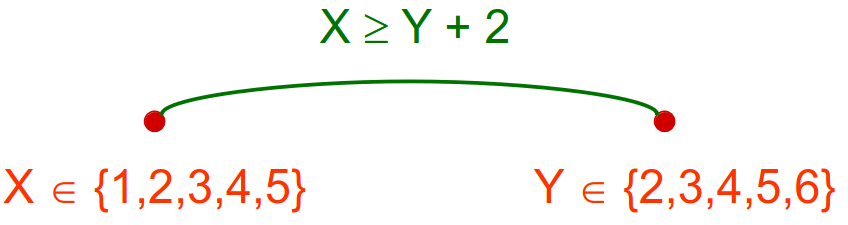
\includegraphics[width=0.7\textwidth]{img/arc.png}
					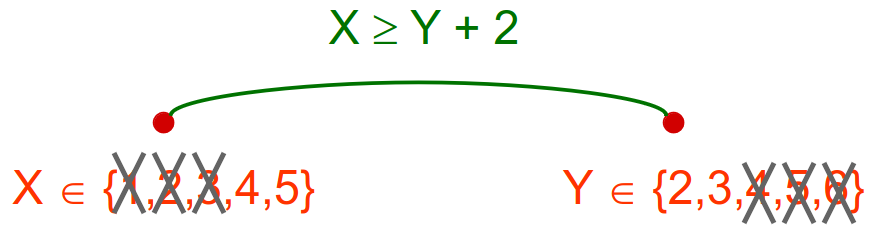
\includegraphics[width=0.7\textwidth]{img/arc1.png}
				\end{figure}
			\item \textbf{Path Consistency} : on considère des contraintes entre $n$ variables
		\end{itemize}
				
		\textbf{Bound consistency : }
			Une forme plus faible de \textit{Arc consistency}. On considère seulement les limites du domaine, donc on retire toujours les valeurs sur les limites et jamais au milieu
			
		\textbf{Global consistency : }
			Pour les contraintes spéciales, c'est géré avec un "ad hoc specialized method". pour un nombre arbitraire de variable
			
		\subsubsection{Arc-consistency algorithm}
			\begin{figure}[htp]
				\centering
				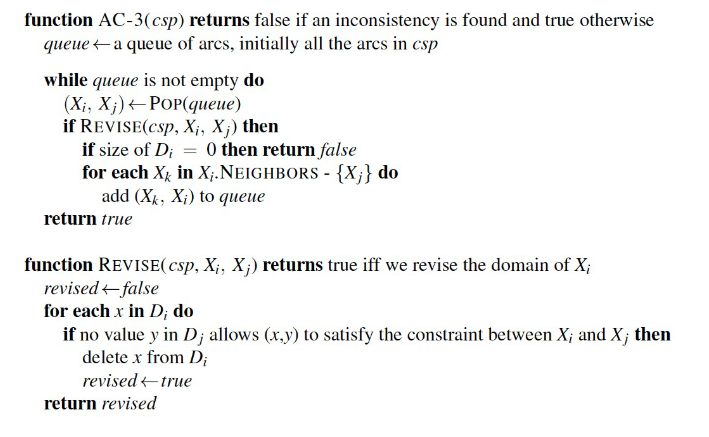
\includegraphics[width=0.7\textwidth]{img/AC-3.png}
			\end{figure}
			
			Avec une complexité de $\mathcal{O}(n^2d^3)$
			
			un peu d'explication :
			\begin{enumerate}
				\item on commence un queue avec un arc initial
				\item temps que il y a $(X_i,X_j)$ dans la queue
				\item si \textit{REVISITE}
				\item alors pour tous les valeurs voisine de $X_i$ sans compter $X_j$, on ajoute $(X_k,X_i)$ dans la queue
			\end{enumerate}
			
			\textit{REVISITE} supprime toutes les valeurs dans $X_i$ tels que elles ne satisfont pas les contrainte entre $X_i$ et $X_j$.
			
	\subsection{Backtracking Search for CSPs}
		\subsubsection{Incremental formulation}
			\begin{itemize}
				\item le \textbf{Init state} est une affectation vide
				\item La \textbf{fonction de succession} assigne une valeur a une variable non assignée si aucune contrainte est violé
				\item Le \textbf{Goal test} verifie si l'affectation actuelle est complete
				\item Le \textbf{Path cost} Valeur constante pour chaque etapes qui indique le coup/profondeur du path
			\end{itemize}
			
			L'arbre de recherche a une profondeur de $n$ (nombre de variables) et le nombre de state possible est $\mathcal{O}(d^n)$ avec d la taille du domaine.
			
			La taille de l'arbre est de $\mathcal{O}(n! d^n)$ en raison que le premier niveau est $n.d$ , le deuxieme $(n-1).d$ etc.
			
			CSP seach algo doit seulement considerer une seule variables pour le successeur a chaque node car avec la \textbf{commutativité} quand on assigne une valeur a une variable, nous obtenons la même affectation partielle quel que soit l'ordre
			
		\subsubsection{Backtracking search}
			c'est une recherche par DFS qui choisis une valeur pour une variables et qui reviens en arrière quand une variable plus de valeur qui ne viole pas les contrainte disponibles
		
			\begin{figure}[htp]
				\centering
				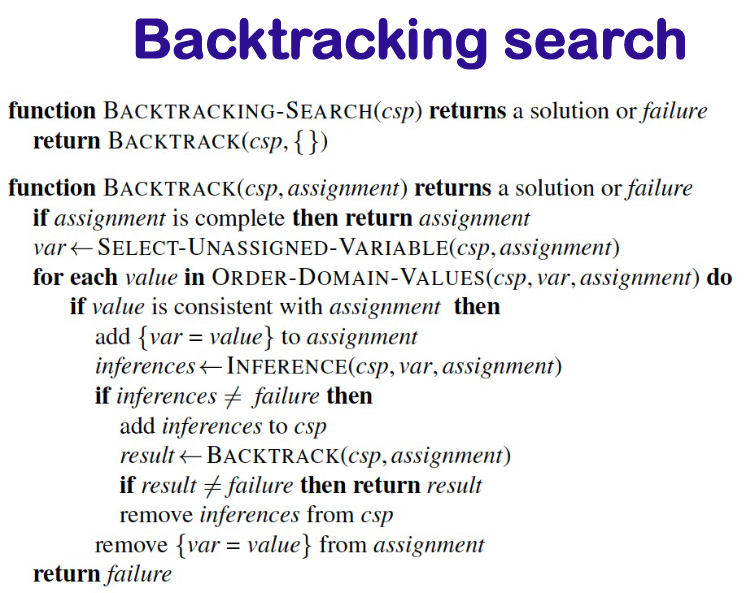
\includegraphics[width=0.7\textwidth]{img/backtrackingSearch.png}

			\end{figure}
			
			\vfill
			
			\begin{figure}[htp]
				\centering
				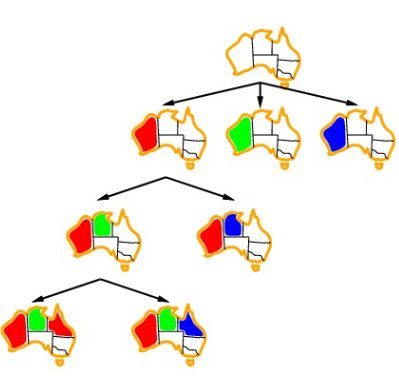
\includegraphics[width=0.5\textwidth]{img/exempleBTS.png}

			\end{figure}
			
		\subsubsection{Variable ordering}
	
			On va optimiser le fait de choisir des variables et des valeurs le tous afin de réduire la recherche
			\begin{itemize}
				\item Minimum Remaining Value (MRV) : on choisis la variable avec le moins de valeur légale
				\item Degree heuristic : on choisis la variables qui entraine le plus grand nombre de contrainte (reduis le facteur de branchement)
			\end{itemize}
			
			\begin{figure}[htp]
				\centering
				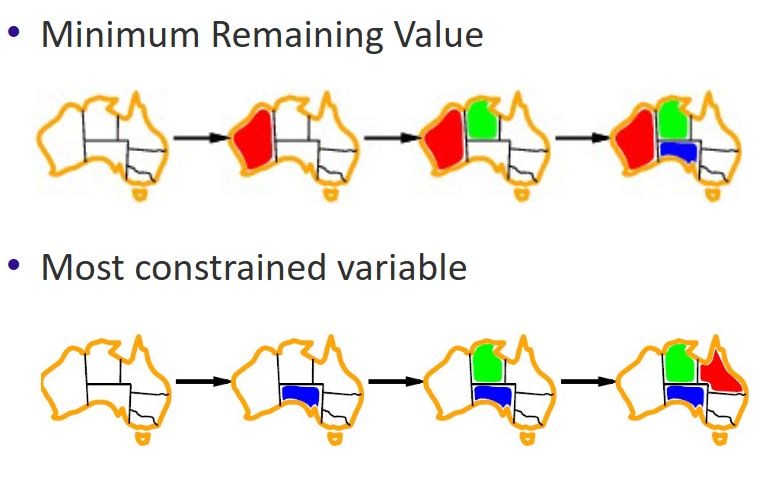
\includegraphics[width=0.5\textwidth]{img/exVarOrd.png}

			\end{figure}
			
		\subsubsection{Interleaving search and inference}
			On veut réduire le \textit{Search Space} pour être plus efficace. Lorsque nous choisissons une valeur pour une variable, nous avons une toute nouvelle possibilité de déduire de nouvelles réductions de domaine sur les variables voisines.
			
			\textbf{Forward checking} : Quand $X$ est attribué a $v$:
			\begin{itemize}
				\item On regarde a chaque variables $T$ non assignées qui sont connectées a $X$
				\item Retirer du domaine $Y$ la valeur incompatible avec la valeur choisie pour $X$.
				
			\end{itemize}
		\subsubsection{Intelligent Backtracking}
			Au lieu de faire un bon en arrière quand on arrive bloquer, on back up a la variables responsable du problème (calculable avec forward checking)
			On garde un \textbf{conflic set} qui garde pour chaque valeur garde l'assignation qui est en conflit avec la valeur.
			
	\subsection{Local Search for CSP}
		\subsubsection{Complete state formulation}
			\begin{itemize}
				\item \textbf{Initial state} : une valeur a chaque variables
				\item \textbf{Sucessor function} : change la valeur d'une variables
				\item \textbf{Goal test} : check si assignement actuelle est consistant et complet
				\item \textbf{Path cost} : Valeur constante par etapes 
			\end{itemize}
			
			Quand on choisie un valeur pour les variables, on choisis avec le minimums de conflit possible
			
		\subsubsection{Min Conflict}
		
			\begin{figure}[htp]
				\centering
				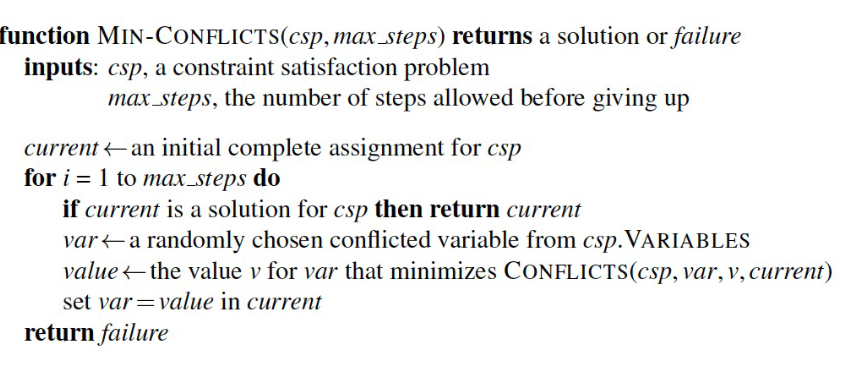
\includegraphics[width=0.8\textwidth]{img/MinConflict.png}
			\end{figure}
			
	\subsection{Structure of the problems}
		\subsubsection{Independent subproblems}
			On divise le CSP en sous-problème indépendant entre eux pour ainsi former $k$ CSP différents. On peut les résoudres séparément et la solution est donc l'unions des différente solutions. 
		
		Avec ça, le complexité temporelle est de $\mathcal{O}(d^{n/k}k)$
			
		\subsubsection{Tree-structure Subproblems}
		
			Si le tree est \textit{directed arc consistency} il peut etre résolué en $\mathcal{O}(nd^2)$
			
			Pour le transformer en tree :
			\begin{itemize}
				\item : retire des nodes :
				\begin{itemize}
					\item choisis un sous-ensemble $S$ de taille $c$
					\item pour chaque assignement possible aux variables de S qui s'attisfonts toutes les contraintes dans $S$,
					\begin{itemize}
						\item Retire dans le domaine, n'importe quelle variables qui sont incohérente avec l'assignement de $S$,
						\item Si CSP a une solution, on la retourne avec assignement $S$
					\end{itemize}
				\end{itemize}
				\item Grouper les nodes:
				\begin{itemize}
					\item chaque variable apparait au moins une fois dans un sous-problème
					\item 2 variables connectées par une contrainte doivent etres ensembles dans au moins un sous-problème
					\item si une variables apparais dans 2 sous-problèmes, alors elle doit etre dans tous les sous-problèmes sur le path pour connecté tous les sous-problème.
				\end{itemize}
			\end{itemize}